\documentclass[xetex,mathserif,serif,aspectratio=169]{beamer}

\usepackage{xltxtra}
\usepackage{color}
\usepackage{url}
\usepackage{listings}
\usepackage{fontspec}
\usepackage{geometry}
\usepackage{lastpage}
\usepackage{fancyhdr}
\usepackage{amsmath}
\usepackage{amsthm}
\usepackage{amssymb}
\usepackage{blkarray}
\usepackage{multicol}
\usepackage{relsize}
\usepackage{listings}
\usepackage{xunicode}
\usepackage{xltxtra}
\usepackage{color}
\usepackage{url}
\usefonttheme[onlymath]{serif}

\definecolor{solarized@base03}{HTML}{002B36}
\definecolor{solarized@base02}{HTML}{073642}
\definecolor{solarized@base01}{HTML}{586e75}
\definecolor{solarized@base00}{HTML}{657b83}
\definecolor{solarized@base0}{HTML}{839496}
\definecolor{solarized@base1}{HTML}{93a1a1}
\definecolor{solarized@base2}{HTML}{EEE8D5}
\definecolor{solarized@base3}{HTML}{FDF6E3}
\definecolor{solarized@yellow}{HTML}{B58900}
\definecolor{solarized@orange}{HTML}{CB4B16}
\definecolor{solarized@red}{HTML}{DC322F}
\definecolor{solarized@magenta}{HTML}{D33682}
\definecolor{solarized@violet}{HTML}{6C71C4}
\definecolor{solarized@blue}{HTML}{268BD2}
\definecolor{solarized@cyan}{HTML}{2AA198}
\definecolor{solarized@green}{HTML}{859900}
\definecolor{yaleblue}{HTML}{0E4C92}

\newcommand{\yellow}[1]{\textcolor{solarized@yellow}{#1}}
\newcommand{\orange}[1]{\textcolor{solarized@orange}{#1}}
\newcommand{\red}[1]{\textcolor{solarized@red}{#1}}
\newcommand{\magenta}[1]{\textcolor{solarized@magenta}{#1}}
\newcommand{\violet}[1]{\textcolor{solarized@violet}{#1}}
\newcommand{\blue}[1]{\textcolor{solarized@blue}{#1}}
\newcommand{\cyan}[1]{\textcolor{solarized@cyan}{#1}}
\newcommand{\green}[1]{\textcolor{solarized@green}{#1}}
\newcommand{\yblue}[1]{\textcolor{yaleblue}{#1}}
\newcommand{\base}[1]{\textcolor{solarized@base01}{#1}}


\defaultfontfeatures{Mapping=tex-text}
\hypersetup{pdfstartview={FitH}}

\newcommand{\old}[1]{\fontspec[Alternate=1,Ligatures={Common}]{Hoefler Text}\fontsize{18pt}{30pt}\selectfont #1}%
\newcommand{\oldA}[1]{\fontspec[Alternate=1,Ligatures={Common, Rare}]{Hoefler Text}\fontsize{12pt}{15pt}\selectfont #1}%
\newcommand{\oldB}[1]{\fontspec[Ligatures={Common}]{Didot}\fontsize{12pt}{15pt}\color{solarized@base02}\selectfont #1}%
\newcommand{\tfont}[1]{\fontspec[Alternate=1,Ligatures={Common}]{Hoefler Text}\fontsize{12pt}{20pt}\selectfont #1}%
\newcommand{\dfont}[1]{\fontspec[Ligatures={Common}]{Didot}\fontsize{12pt}{12pt}\selectfont #1}%

\setbeamerfont{title}{family=\old}
\setbeamerfont{author}{family=\tfont}%
\setbeamerfont{frametitle}{family=\oldA}
\setbeamerfont{date}{family=\dfont}

\setbeamertemplate{navigation symbols}{}
\setbeamertemplate{footline}[text line]{%
  \parbox{0.99\linewidth}{
    \normalsize\vspace*{-24pt}\hfill{\color{solarized@base00}\insertframenumber/\inserttotalframenumber}
  }
}


\setlength{\parindent}{0pt}
\setlength{\parskip}{12pt}

\setbeamercolor{structure}{bg=solarized@base3, fg=solarized@base02}
\setbeamercolor{titlelike}{fg=solarized@cyan}
\setbeamercolor{title}{fg=solarized@blue}
\setbeamercolor{subtitle}{fg=solarized@magenta}
\setbeamercolor{alerted text}{fg=orange}
\setbeamercolor{itemize}{fg=solarized@base02}
\setbeamercolor{background canvas}{bg=solarized@base3}
\setbeamercolor{enumerate subitem}{fg=solarized@base02}

\newcommand{\minimize}{\mathop{\mathrm{minimize}}}
\newcommand{\argmin}{\mathop{\mathrm{arg\,min}}}
\newcommand{\argmax}{\mathop{\mathrm{arg\,max}}}
\newcommand{\st}{\mathop{\mathrm{subject\,\,to}}}


\usepackage[]{algorithm2e}
\usepackage{../kbordermatrix}

\begin{document}

%%%%%%%%%%%%%%%%%%%%%%%%%%%%%%%%%%%%%%%%%%%%%%%%%%%
\begin{frame}[fragile] \frametitle{} \oldB \small

\vfill

{\fontsize{0.7cm}{0cm}\selectfont Lecture 13 \\\vspace{0.2cm} Back-propagation}\\\vspace{0.5cm}
02 March 2016

\vspace{2cm}

\begin{minipage}{0.6\textwidth}
Taylor B. Arnold \\
Yale Statistics \\
STAT 365/665
\end{minipage}
\hfill
\begin{minipage}{0.3\textwidth}\raggedleft

\includegraphics[scale=0.3]{../yale-logo.png}
\end{minipage}%

\end{frame}

%%%%%%%%%%%%%%%%%%%%%%%%%%%%%%%%%%%%%%%%%%%%%%%%%%%
\begin{frame}[fragile] \frametitle{} \oldB \small

Notes:
\begin{itemize}
\item Problem set 4 is due this Friday
\item Problem set 5 is due a week from Monday (for those of you
with a midterm crunch this week); I will post the questions by
tomorrow morning
\end{itemize}

\end{frame}

%%%%%%%%%%%%%%%%%%%%%%%%%%%%%%%%%%%%%%%%%%%%%%%%%%%
\begin{frame}[fragile] \frametitle{} \oldB \small

\yblue{\textbf{Neural network review}}

Last time we established the idea of a sigmoid neuron,
which takes a vector of numeric variables $x$ and emits
a value as follows:
\begin{align*}
\sigma(x \cdot w + b) &= \frac{1}{1 + e^{-(x \cdot w + b)}}
\end{align*}
It is entirely defined by a vector of weights $w$ and bias term $b$,
and functions exactly like logistic regression.

\end{frame}

%%%%%%%%%%%%%%%%%%%%%%%%%%%%%%%%%%%%%%%%%%%%%%%%%%%
\begin{frame}[fragile] \frametitle{} \oldB \small

\yblue{\textbf{Neural network review, cont.}}

These single neurons can be strung together to construct a neural
network. The input variables are written as special neurons on the
left-hand side of the diagram:

\begin{center}
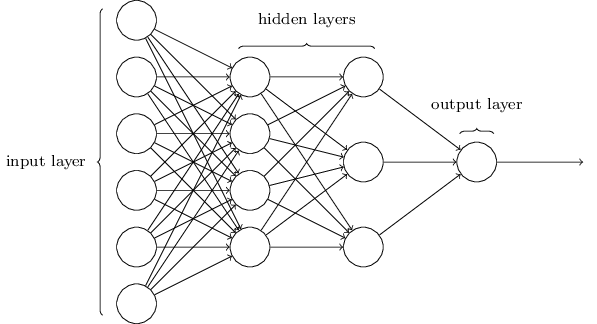
\includegraphics[height=4cm]{img/tikz11.png}
\end{center}

\end{frame}

%%%%%%%%%%%%%%%%%%%%%%%%%%%%%%%%%%%%%%%%%%%%%%%%%%%
\begin{frame}[fragile] \frametitle{} \oldB \small

\yblue{\textbf{Stochastic gradient descent}}

We started talking about how to learn neural networks via a variant
of gradient descent, called \blue{stochastic gradient descent}. The
only detail left to figure out is exactly how calculate the gradient
of the cost function in an efficient way.

\end{frame}

%%%%%%%%%%%%%%%%%%%%%%%%%%%%%%%%%%%%%%%%%%%%%%%%%%%
\begin{frame}[fragile] \frametitle{} \oldB \small

\yblue{\textbf{Idea behind back-propagation}}

Before starting down the path of explaining the math behind
back-propagation, I want to explain what the big idea behind
the method is and why it makes sense as a general approach.

\end{frame}

%%%%%%%%%%%%%%%%%%%%%%%%%%%%%%%%%%%%%%%%%%%%%%%%%%%
\begin{frame}[fragile] \frametitle{} \oldB \small

\yblue{\textbf{Idea behind back-propagation, cont.}}

\begin{center}
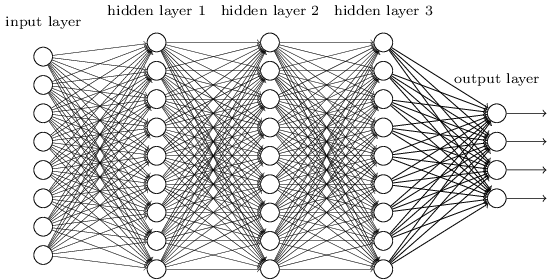
\includegraphics[height=6cm]{img/tikz40.png}
\end{center}

\end{frame}

%%%%%%%%%%%%%%%%%%%%%%%%%%%%%%%%%%%%%%%%%%%%%%%%%%%
\begin{frame}[fragile] \frametitle{} \oldB \small

\yblue{\textbf{Some notation, cont.}}

We need a way of referring unambiguously to the weights and biases
in a multi-layer neural network. To start define

\vspace{-0.5cm}
{\Huge
\begin{align*}
\blue{w^{l}_{j,k}}
\end{align*}
}

As the weight of node k in layer $l-1$ as applied by node j in
layer $l$.

\end{frame}

%%%%%%%%%%%%%%%%%%%%%%%%%%%%%%%%%%%%%%%%%%%%%%%%%%%
\begin{frame}[fragile] \frametitle{} \oldB \small

\yblue{\textbf{Some notation, cont.}}

Now let:

\vspace{-0.5cm}
{\Huge
\begin{align*}
\magenta{b^l_j}
\end{align*}
}

Be the bias of node $j$ of layer $l$.

\end{frame}

%%%%%%%%%%%%%%%%%%%%%%%%%%%%%%%%%%%%%%%%%%%%%%%%%%%
\begin{frame}[fragile] \frametitle{} \oldB \small

\yblue{\textbf{Some notation, cont.}}

We now define two additional quantities. The weighted input
emitted from node $j$ in layer $l$:

\vspace{-0.5cm}
{\Huge
\begin{align*}
\violet{z^l_j}
\end{align*}
}

The term input refers to the fact that this in the input to
the activation function.

\end{frame}

%%%%%%%%%%%%%%%%%%%%%%%%%%%%%%%%%%%%%%%%%%%%%%%%%%%
\begin{frame}[fragile] \frametitle{} \oldB \small

\yblue{\textbf{Some notation, cont.}}

And the activation

\vspace{-0.5cm}
{\Huge
\begin{align*}
\yellow{a^l_j}
\end{align*}
}

Derived from applying the function $\sigma$ (the sigmoid or logit function
for us so far) to the the weighted input \violet{$z^l_j$}.

\end{frame}

%%%%%%%%%%%%%%%%%%%%%%%%%%%%%%%%%%%%%%%%%%%%%%%%%%%
\begin{frame}[fragile] \frametitle{} \oldB \small

\yblue{\textbf{Some notation, cont.}}

That's a lot to take in all at once. Here is the cheat-sheet version
that shows how all of these quantities fit together:
\begin{align*}
\yellow{a^l_j} &= \sigma(\violet{z^l_j}) \\
&= \sigma(\sum_k \blue{w^l_{jk}} \yellow{a_k^{l-1}} + \magenta{b^l_j})
\end{align*}
\pause It will, also, be beneficial to define one more quantity:
\begin{align*}
\cyan{\delta_j^l} &= \frac{\partial C}{ \partial z_j^l}
\end{align*}
Called the error functions. These error functions will help in keeping the
number of computations we need to make as small as possible.

\end{frame}

%%%%%%%%%%%%%%%%%%%%%%%%%%%%%%%%%%%%%%%%%%%%%%%%%%%
\begin{frame}[fragile] \frametitle{} \oldB \small

\yblue{\textbf{Cost function again}}

In what follows we assume that we are dealing with one individual
data point. So the cost is simply the cost of that one training
point (which we called $C_i$ in Monday's notes).

If the neural network has $L$ total layers, notice that in
general we will have the cost being a function only of the
activations from layer $L$ of the neural network:
\begin{align*}
C(w, b) &= f(a_1^L, a_2^L, \ldots)
\end{align*}
In our case, this can be explicitly written as:
\begin{align*}
C(w, b) &= \sum_k (y_k - a_k^L)^2
\end{align*}
Note: this sum is over the dimension of the output, not the
number of samples! If we only have a univariate output, this
will just be a single value.

\end{frame}

%%%%%%%%%%%%%%%%%%%%%%%%%%%%%%%%%%%%%%%%%%%%%%%%%%%
\begin{frame}[fragile] \frametitle{} \oldB \small

\yblue{\textbf{Feed-forward step}}

We want to calculate how much the cost changes with respect to the
errors on the outer layer. This ends up being a fairly straightforward
application of the chain rule:
\begin{align*}
\delta_j^L &= \frac{\partial C}{ \partial z_j^L} \\
&= \sum_k \frac{\partial C}{ \partial a_k^L} \cdot \frac{\partial a_k^L}{ \partial z_j^L} \\
&= \frac{\partial C}{ \partial a_j^L} \cdot \frac{\partial a_j^L}{ \partial z_j^L} \\
&= \frac{\partial C}{ \partial a_j^L} \cdot \sigma'(z_j^L)
\end{align*}

\end{frame}

%%%%%%%%%%%%%%%%%%%%%%%%%%%%%%%%%%%%%%%%%%%%%%%%%%%
\begin{frame}[fragile] \frametitle{} \oldB \small

\yblue{\textbf{Feed-forward step, cont.}}

We can explicitly calculate the first partial derivative given the cost
function. Here for example it is given as:
\begin{align*}
\frac{\partial C}{ \partial a_j^L} &= \frac{\partial}{ \partial a_j^L} \sum_k (y_k - a_k^L)^2 \\
&= 2 \cdot (a_j^L - y_j)
\end{align*}
The function $\sigma'$ is also easily determined by differentiation of the sigmoid
function:
\begin{align*}
\sigma'(z) &= \sigma(z) \cdot (1 - \sigma(z))
\end{align*}

\end{frame}

%%%%%%%%%%%%%%%%%%%%%%%%%%%%%%%%%%%%%%%%%%%%%%%%%%%
\begin{frame}[fragile] \frametitle{} \oldB \small

\yblue{\textbf{Back-propagation step}}

We now want to relate the errors $\delta_j^l$ to the errors in $\delta_j^{l+1}$.
This allows us to then work backwards from the feed-forward step.
Notice that:
\begin{align*}
\delta_j^l &= \frac{\partial C}{ \partial z_j^l} \\
&= \sum_k \frac{\partial C}{ \partial z_k^{l+1}} \cdot \frac{\partial z_k^{l+1}}{ \partial z_j^l} \\
&= \sum_k \delta_k^{l+1} \cdot \frac{\partial z_k^{l+1}}{ \partial z_j^l}
\end{align*}
\pause To calculate the remaining derivatives, notice that we have a formula relating
one set of weighted inputs to the next set:
\begin{align*}
z^{l+1}_k &= \sum_{i} w^{l+1}_{ki} a^l_i + b_k^{l+1} \\
&= \sum_i w^{l+1}_{ki} \sigma(z_i^l) + b_k^{l+1}
\end{align*}

\end{frame}

%%%%%%%%%%%%%%%%%%%%%%%%%%%%%%%%%%%%%%%%%%%%%%%%%%%
\begin{frame}[fragile] \frametitle{} \oldB \small

\yblue{\textbf{Back-propagation step, cont.}}

Using this relationship, we can now take partial derivatives
\begin{align*}
\frac{\partial z^{l+1}_k}{ \partial z^{l}_j}
&= \frac{\partial}{ \partial z^{l}_j} \left( \sum_i w^{l+1}_{ki} \sigma(z_j^l) + b_k^{l+1} \right) \\
&= w^{l+1}_{kj} \cdot \sigma'(z_j^l)
\end{align*}
Which when plugged into our original equations yields:
\begin{align*}
\delta_j^l &= \sum_k \delta_k^{l+1} \cdot w^{l+1}_{kj} \cdot \sigma'(z_j^l)
\end{align*}

\end{frame}

%%%%%%%%%%%%%%%%%%%%%%%%%%%%%%%%%%%%%%%%%%%%%%%%%%%
\begin{frame}[fragile] \frametitle{} \oldB \small

\yblue{\textbf{Relating errors to weights and bias}}

We now just need to relate the errors $\delta_j^l$ to the
gradient with respect to the weights and biases directly.
We have, from the linearity of the bias term, a very simple
relationship between $\delta_j^l$ with the gradient of
the bias terms:
\begin{align*}
\delta_j^l &= \frac{\partial C}{ \partial z_j^l} \\
&=\frac{\partial C}{ \partial b_j^l} \cdot \frac{\partial b_j^l}{ \partial z_j^l} \\
&=\frac{\partial C}{ \partial b_j^l}
\end{align*}


\end{frame}


%%%%%%%%%%%%%%%%%%%%%%%%%%%%%%%%%%%%%%%%%%%%%%%%%%%
\begin{frame}[fragile] \frametitle{} \oldB \small

\yblue{\textbf{Relating errors to weights and bias}}

For the weights, a very similar
\begin{align*}
\delta_j^l &= \frac{\partial C}{ \partial z_j^l} \\
&=\frac{\partial C}{ \partial w_{jk}^l} \cdot \frac{\partial w_{jk}^l}{ \partial z_j^l} \\
&=\frac{\partial C}{ \partial  w_{jk}^l} \cdot \frac{1}{a^{l-1}_k}
\end{align*}
Which can be re-written as:
\begin{align*}
\frac{\partial C}{ \partial w_{jk}^l} &= a^{l-1}_k \delta_j^l
\end{align*}

\end{frame}


%%%%%%%%%%%%%%%%%%%%%%%%%%%%%%%%%%%%%%%%%%%%%%%%%%%
\begin{frame}[fragile] \frametitle{} \oldB \small

\yblue{\textbf{Putting these all together}}

We have now four equations that describe the mechanics of back-propagation.
I will write them here a bit more compactly for reference:
\begin{align*}
\delta_j^L &= \nabla_{a^L} C \circ \sigma'(z^L) \\
\delta_j^l &= ((w^{l+1})^T \delta^{l+1}) \circ \sigma'(z^l) \\
\frac{\partial C}{\partial b^l_j} &= \delta^l_j \\
\frac{\partial C}{\partial w^l_{jk}} &= a^{l-1}_k \delta^l_j
\end{align*}
Where dropping an index indicates that I am doing math on the entire vector
or matrix of values. The symbol $\circ$ (Hadamard product)
refers to element-wise multiplication; a common operation in programming
but less-so in abstract mathematics.

\end{frame}

%%%%%%%%%%%%%%%%%%%%%%%%%%%%%%%%%%%%%%%%%%%%%%%%%%%
\begin{frame}[fragile] \frametitle{} \oldB \small

\yblue{\textbf{The back-propagation algorithm}}

The back-propagation algorithm as a whole is then just:
\begin{enumerate}
\item Select an element $i$ from the current minibatch and calculate the weighted
inputs \violet{$z$} and activations \yellow{$a$} for every layer using a forward
pass through the network
\item Now, use these values to calculate the errors $\cyan{\delta}$ for each
layer, starting at the last hidden layer and working backwards, using back-propagation
\item Calculate $\nabla_w C_i$ and $\nabla_b C_i$ using the last two equations
\item Repeat for all samples in the minibatch, to get:
\begin{align*}
\frac{\sum_{i \in M} \nabla_w C_i}{|M|} \approx \nabla_w C \quad \quad \quad
\frac{\sum_{i \in M} \nabla_b C_i}{|M|} \approx \nabla_b C
\end{align*}
\item Update the weights and biases by (the estimates of) $-\eta \cdot \nabla_w C$ and
$-\eta \cdot \nabla_b C$, respectively
\item Repeat over every mini-batch, and for the desired number of epochs
\end{enumerate}

\end{frame}

\end{document}











